%!TeX root=main.tex

% Check data center component or network component, do not mix the two

\section{Problem Formulation}
\label{sec:problem_formulation}

In this section, we start with a descriptive statement of the VNFPP. Then, we give the formal definition of the multi-objective VNFPP considered in this paper followed by an analysis of its feasible search space.

\subsection{Problem Statement}
\label{sec:statement}

A data center consists of a large number servers, each of which can accommodate a limited number of VMs. Traffic is transmitted between servers across the network topology, i.e., a set of switches that interconnect all servers as an example shown in~\pref{fig:topology}. Traffic between VMs on the same server communicate via a virtual switch on the server. In this paper, we refer to the servers and switches, which constitute a data center, as the data center components.

\begin{figure}[t]
	\centering
	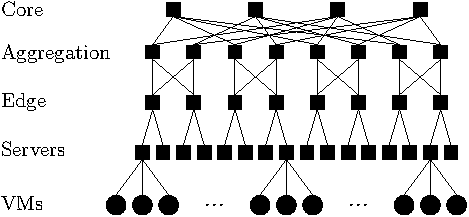
\includegraphics{figures/fat_tree-crop}
	\caption{An NFV enabled Fat Tree network topology with 4 ports and 3 VMs per server.}
	\label{fig:topology}
\end{figure}

A solution to a VNFPP specifies one or more paths through the network topology for each service. In particular, a path is a sequence of data center components that visit each VNF of a service in a prescribed order. Furthermore, each solution also specifies the amount of traffic that should be sent along each path.

The goal of the VNFPP is to provide a number of services by placing VNFs on VMs in the data center and defining the paths so as to maximize QoS and minimize capital and operational costs. In this paper, we formulate a three-objective VNFPP that takes two QoS metrics (i.e., latency and packet loss) and a cost metric (i.e., energy consumption) into account. An understanding of how the QoS and energy consumption interact is critical to the good operation of a data center. A multi-objective formulation of the VNFPP that considers how these metrics conflict informs the decision maker on the possible opportunities that are available. For example, a solver for a multi-objective formulation of the VNFPP enables the data center operator to:
\begin{itemize}
	\item Understand the cost-benefit trade off when increasing the amount of resources spent on services.
	\item Investigate how parameters such as network topology and the properties of servers and services could affect these trade offs.
	\item Make an informed selection from the set of possible trade off solutions.
\end{itemize}

%\begin{table}[t]
%	\caption{Lookup table of mathematical notations}
%	\label{tab:definition}
%	\center
%	\begin{tabular}{c|l}
%		\hline
%		Symbol & Definition \\
%		\hline
%        $\mathcal{S}$     & Set of all services \\
%        $\mathcal{C}$     & Set of all network components \\
%        $\mathcal{C}^{s}$ & Set of all servers \\
%        $\mathcal{V}$     & Set of all VNFs \\
%        $\mathcal{L}$     & Set of links connecting network components\\
%        $\mathcal{R}^s$   & Set of all routes for the service $s$ \\
%		$\mathcal{A}$     & Set of anti-affinity services \\
%		\hline
%		$\mathbb{P}^d_s$ & Service packet loss probability \\
%		$\mathbb{P}_{R^s_i}$ & The probability the route $R^s_{i}$ is taken \\
%		$\mathbb{P}^d_c$ & Component packet loss probability \\
%		$R^s_{i}$       & The $i$th route for service $s$ \\
%		$R^s_{i,j}$     & The $j$th component of the $i$th route of service $s$ \\
%		$W_s$ & Service latency \\
%		$\lambda_s$ & Service arrival rate \\
%		$\lambda_c$ & Component arrival rate \\
%		$\mu_c$ & Component service rate \\
%		$B_c$ & Component queue length $c$ \\
%		$\mathbb{W}_c$ & Component waiting time \\
%        \hline
%		$\gamma$ & Model threshold \\
%		$\Delta$ & Number of iterations below threshold \\ 
%
%		$N^M_v$ & Max number of instances of the VNF $v$ \\
%
%		$|\cdot|$ & Cardinality of a set or sequence \\
%		\hline
%	\end{tabular}
%\end{table}

\subsection{Mathematical Formulation}
\label{sec:formulation}

We first list some core terminologies important to the mathematical formulation of the objective and constraint functions of the VNFPP in this paper. $\mathcal{S}$ is the set of services that must be placed and $\mathcal{V}$ is the set of VNFs. A service $s=\{s_1,\cdots,s_n\}\in\mathcal{S}$ is a sequence of VNFs. The network topology is represented as a graph $\mathcal{G}=(\mathcal{C},\mathcal{L})$, where $\mathcal{C}$ denotes the set of data center components and $\mathcal{L}$ denotes the set of links connecting them. A route is a sequence of data center components where $\mathcal{R}^s$ is the set of paths for $s$, $R_{i}^s$ is the $i$th path of $s$ and $R_{i,j}^s$ is the $j$th component of this path. The complete notations are listed in Table I of Appendix A\footnote{The appendix document can be downloaded from \url{here}.}. %Finally, $|\cdot|$ indicates the cardinality of a set or a sequence. 

Overall, the VNFPP considered in this paper is defined as a MOP of the following three metrics.
\begin{itemize}
	\item The \textit{total energy consumption} (denoted as $E_C$).
	\item The \textit{mean latency} of the services (denoted as $L$):
	      \begin{equation}
		      L=\sum_{s\in\mathcal{S}} W_{s}/|\mathcal{S}|,
	      \end{equation}
	      where $W_s$ is the expected latency of $s\in\mathcal{S}$.
	\item The \textit{mean packet loss} of the services (denoted as $P$):
	      \begin{equation}
		      P=\sum_{s\in\mathcal{S}} \mathbb{P}^d_s/|\mathcal{S}|,
	      \end{equation}
	      where $\mathbb{P}^d_s$ is the packet loss probability of $s\in\mathcal{S}$.
\end{itemize}
In addition, there are five constraints associated with this VNFPP. Three of them are core constraints applicable to any VNFPP and are defined as follows.%The analytical modeling of these three metrics will be derived in~\pref{sec:system_model}.
\begin{itemize}
	\item Sequential data center components in a route must be connected by an edge:
	      \begin{equation}
		      (R_{i,j}^s, R_{i,j+1}^s) \in \mathcal{L}.
	      \end{equation}
	\item Each server can accommodate up to $N^V$ VNFs:
	      \begin{equation}
		      \sum_{v\in\mathcal{V}} A_v^{c_{\mathsf{s}}}<N^V,
	      \end{equation}
	      where $A_v^{c_{\mathsf{s}}}$ is the number of instances of the VNF $v$ assigned to the server ${c_{\mathsf{s}}}$.
	\item All VNFs must appear in the route and in the order defined by the service:
	      \begin{equation}
		      \pi^{R^s}_{s_i}\neq\emptyset,\quad\pi^{R_i}_{s_i}<\pi^{R_i}_{s_{i+1}},
	      \end{equation}
	      where $\pi^{R_i}_{s_i}$ is the index of the VNF $s_i$ in the route $R_i$.
\end{itemize}

In practice, security and legal concerns can impose additional constraints.
\begin{itemize}
	\setcounter{enumi}{3}
	\item A business may require an exclusive access to the servers in use due to security or performance restrictions. These requirements can be expressed through \textit{anti-affinity constraints} that restrict which services can share servers. For each service $s\in\mathcal{A}$ where $\mathcal{A}$ is the set of anti-affinity services, the anti-affinity constraints are defined as:
	      \begin{equation}
		      A^{c_{\mathsf{s}}}_{v_1}\cdot A^{c_{\mathsf{s}}}_{v_2}=0,\quad\forall v_1\in s, v_2\notin s.
	      \end{equation}

	\item VNFs may be provided under a license that restricts the number of instances of a VNF that can be created. These are known as the \textit{max instance constraints}:
	      \begin{equation}
		      \sum_{c_s\in\mathcal{C}^s} A_v^{c_{\mathsf{s}}}\leq N_v^M,
		      \label{eq:max_instances}
	      \end{equation}
	      where $N^M_v$ is the maximum number of instances of the VNF $v$ and $\mathcal{C}^{s}$ is the set of all servers.
\end{itemize}

The combination of the constraints and objectives results in a challenging optimization problem. Although each of the constraints can be considered independently, each constraint is complex such that the feasible search space is small relative to the overall search space. Further, the NP-Hardness of the problem means that the feasible search space still contains many solutions, few of which will be at or near optimal.

\subsection{Analysis of Feasible Search Space}
\label{sec:complexity}

It is acknowledged that VNFPP is a NP-hard problem~\cite{CohenLNR15,LuizelliCBG17,SangJGDY17} with various constraints. However, the relative size of the feasible region against the entire space has been overlooked in the literature. A small feasible region can make it significantly difficult to find feasible solutions, let alone optima.

In the context of VNFPP, a solution is feasible if at least one instance of every VNF has been placed. Here we plan to verify that the relative size of the feasible region, which is the probability of a randomly selected solution being feasible, is small. However, due to the NP-hardness of the VNFPP, there is no closed form solution of this relative size. Therefore, we estimate an upper bound instead. In particular, we consider the case where each VNF can be placed at any location independent of whether other VNFs have been placed therein. In the following paragraphs, we first verify that this is indeed an upper bound and then we provide a quantitative estimation to show that it is proportionately small.

\begin{lemma}
	The feasible region under the independence assumption is larger than the exact feasible region.\footnote{The proof can be found in the Appendix B.}
\end{lemma}

%\begin{proof}
%The independence assumption allows each VNF to be placed at any location independently of where other VNFs have been placed. We refer to the feasible region under the independence assumption as the independent feasible region. The independent feasible region contains all solutions where multiple VNFs occupy the same VM. In addition, it also contains all solutions where VNFs are not placed on the same location. This latter subspace is the exact feasible region and a subset of the independent feasible region.
%\end{proof}

Based on the independence assumption, the probability of a VNF being placed is calculated as:
\begin{equation}
	\mathbb{P}^p_{v}=1-\left(1-\frac{1}{|\mathcal{V}|}\right)^N,
\end{equation}
where $N$ is the number of VMs. Hence, the probability at least one VNF is not placed is calculated as:
\begin{equation}
	\mathbb{P}^{\neg p}=1-\left(\mathbb{P}^p_v\right)^{\mathcal{V}}.
\end{equation}
\pref{fig:p_feasible} plots the probability of generating a feasible solution for a data center with different capacities. From these trajectories, we find that the ratio of the feasible region against the entire search space approaches zero even for very low utilizations. The anti-affinity and max instance constraints further reduce the size of the feasible region, thus leading to a significantly increased difficulty.
\begin{figure}[t!]
	\centering
	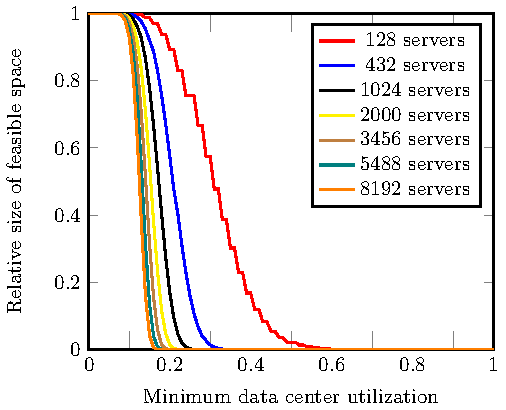
\includegraphics[width=\linewidth]{graphs/general/p_feasible}
	\caption{Demonstration of an upper bound of the proportion of the feasible region for different data center sizes. The proportionate size of the feasible region against the entire search space approaches zero even with a low utilization.}
	\label{fig:p_feasible}
	\vspace{1em}
\end{figure}

%In summary, the VNFPP is challenging not only because of its NP-hardness, but also its extremely small feasible region.
